\chapter{Theoretical Background}\thispagestyle{fancy}
\section{Discrete Dynamical Systems}

\paragraph*{}
Dynamical system theory is a vast field, with various applications in natural and social sciences. It uses all kinds of mathematical concepts from different areas, but to maintain clarity throughout this work, we will only focus on the necessary definitions in this section. In the most general sense the theory is about modeling systems, especially how a certain set of its variables $ \boldsymbol{x} = \{x_1,\dots,x_N\} $ evolves over time. A more precise definition of a set will be given in the next section, but for now it is simply the collection of those variables. 

\paragraph*{}
Classically, the theory of dynamical systems deals only with a hand full of variables. However, in nature, we often have many separate parts that interact with each other. Because of this, the theory of complex systems evolved. With it, theorists try to deduce seemingly complicated collective behavior as an emergent property of the rules the part taking components have to obey. The random Boolean networks (RBNs) on which this thesis is mainly about, can be seen as a prototypical complex system. Many properties can be derived analytically for it and it shows many phenomena other complex systems also have. That is why scientists studied RBNs extensively and many reviews on them have been written by now, for example, M. Aldana et al. \cite{aldana2003boolean} or B. Drossel \cite{drossel2008random}. We will return to them later on when we have provided the necessary knowledge to understand such networks properly.

\paragraph*{Dynamical Systems}
One major separation between different classes of models of dynamical systems is the way how time gets defined. Here it will only be discrete and can be associated with the natural numbers: $ t \in \mathbb{N} $. Let the phase space $ \mathcal{X} $ be the set of all possible values the variables $ \boldsymbol{x} $ can have and define the map $ \phi :  \mathcal{U}\subset\mathcal{X} \longrightarrow \mathcal{X} $ with $ \boldsymbol{x} \mapsto \phi (\boldsymbol{x}) $. It will be chosen in a way, that the following equation then defines the dynamical system and its behavior for all times:
\begin{equation}
\boldsymbol{x}_{t+1} = \phi(\boldsymbol{x}_t).
\end{equation} 
The indices denote the point in time of the variables. This notation is commonly used for systems with discrete-time evolution and will be used equivalently to the continuous one. Thus we will use $ x(t) $ and $ x_t$ interchangeably.

\paragraph*{Fixpoints}
There are many ways the parameters could be evolving. They could, for example, only grow, decrease or do both and maybe oscillate. One interesting thing is fixpoints and limit cycles. If there exists a point $ \boldsymbol{x}^*\in \mathcal{X} $, it will be called a fixpoint, if it fulfills the following equation:
\begin{equation}\label{eq:fixpoint}
\boldsymbol{x}^*=\phi(\boldsymbol{x}^*).
\end{equation}

\paragraph*{}
Once the system reaches this point, it stays for all following time steps at it. If the map $ \phi $ has a first derivative with respect to time, the stability of this fixpoint could be further analyzed analytically. But since this is not always the case, as it happens to be in our model as well, we first want to define stability in a dynamical manner. If there exists at least one $ \boldsymbol{x}_0\in \mathcal{X} $, such that 
\begin{equation}\label{eq:stable_fixpoint}
\lim\limits_{t\rightarrow \infty} \phi^t (\boldsymbol{x}_0) = \boldsymbol{x}^*\text{ and } \boldsymbol{x}_0 \neq \boldsymbol{x}^*,
\end{equation}
the fixpoint will be called stable. This equation is analogous to the notion, that the phase space contracts around $ \boldsymbol{x}^* $ in a continuous time system. Note that the superscript over the map is not a power and means instead $ t $ times its composition:
\begin{equation}
\phi^t (\boldsymbol{x}) := \underbrace{(\phi \circ\dots\circ\phi)}_{t\text{ times}}(\boldsymbol{x}).
\end{equation}

\paragraph*{}
We will continue with the analysis of stability, but first, we have to introduce cycles since their concept is closely related to fixpoints.

\paragraph*{Cycles}
Another possible behavior of the system would be for it coming back to a previous state $ \boldsymbol{x}_1\in \mathcal{X} $ after $ L $ time steps:
\begin{equation}
\boldsymbol{x}_1 = \phi^L(\boldsymbol{x}_1).
\end{equation}
Of course, this implies that $ L $ is the shortest number of steps, where this equation holds. From this chain it is possible to construct the series $ \left(\boldsymbol{x}_1,\phi(\boldsymbol{x}_1),\dots,\phi^{L-1}(\boldsymbol{x}_1) \right) \in \mathcal{X}^L $, which will be called a cycle $ C_L $ of length 
$ L $. It is not important from which state the cycle starts. What matters is its order and size. If equation (\ref{eq:stable_fixpoint}) holds for at least one element of the cycle, then it is also called stable. A cycle with $ L=1 $ is just a fixpoint. The more general term is attractor, whenever we talk about either a stable fixpoint or a stable cycle.

\paragraph*{Stability}
We now apply the phase space with a metric $d : \mathcal{X}\times\mathcal{X} \longrightarrow [0,\infty) $, with which we can measure distances between two elements of it. From it we define the norm as the distance of some element $x$ to the zero element: $\|x\|:=d(0,x)$. We further assume that the phase space is linear and derivations can be properly defined on it. More information on those topics can be found virtually in every introductory course on vector spaces or related topics in the literature, so this is as much as we need to know for now. 

\paragraph*{}
With this, we can further analyze the stability of a found fixpoint $x^*$ for a given dynamical map $\phi$ in a single dimension. Let us say that at time $t$, we are the smallest possible distance away from $x^*$:
\begin{equation}
\Delta x_t := x_t-x^*.
\end{equation}
We use this for a tailor expansion of the evolution map at the fixpoint:
\begin{equation}
\begin{split}
x_{t+1}& = \phi(x_t) = \phi(x^*+\Delta x_t)\\
& = \phi(x^*) + \phi'(x^*)\Delta x_t + O(\Delta x_t^2)\\
& = x^* + \phi'(x^*)\Delta x_t + O(\Delta x_t^2),
\end{split}
\end{equation}

\paragraph*{}
To drop the terms of higher-order $\Delta x_t$ has to be smaller than one, but even if it is not, we can substitute the variables and reformulate the problem in a way where this is given. By doing so, we end up with a relation from which we can deduce the stability of the fixpoint: 
\begin{equation}
\frac{\Delta x_{t+1}}{\Delta x_{t}} = \phi'(x^*).
\end{equation}

\paragraph*{}
If this is smaller than one, our distance to the fixpoint will decrease over time until we arrive at it. Thus we call it stable. If for every time-step, the distance keeps growing, we would call it unstable. To summarize this up, we have:
\begin{equation}\label{eq:fixpoint_stability}
\begin{split}
\|\phi'(x^*)\| < 1 & \Longleftrightarrow x^* \text{ is stable,} \\
\|\phi'(x^*)\| > 1 & \Longleftrightarrow x^* \text{ is unstable.}
\end{split}
\end{equation}

If we get exactly the value of one, we would have to gather additional information. We could maybe try to analyze the fixpoint's stability in the way we introduced its concept earlier and use equation (\ref{eq:stable_fixpoint}). This topic is closely related to the so-called Lyapunov exponents. We could introduce the idea of eigenvalues and how to use them to analyze the system even further. But since we will gain little to no more insights on random boolean networks, which are the main topic of this thesis, we will simply leave it like this and continue with other more relevant definitions.

\section{Probability Theory}
\paragraph*{}
We will later look at large ensembles and assign probabilities to certain properties of them. To define what this means, we will provide a short introduction in this section. There are many modern approaches to probability theory and for a more comprehensive introduction, we refer to the books of  A. Klenke \cite{klenke2013probability} and B. R. Bhat \cite{bhat2007modern}. For our purposes, it is enough to reduce ourselves to naive set theory as our basis.

\paragraph*{Sets}
Any unordered collection of elements will be called a set $\mathcal{S}$. If $x$ is an element in $\mathcal{S}$, we write $x\in \mathcal{S}$. For example and further definition, let $a$ and $b$ form the set $\mathcal{S}:=\{a,b\}$. As such it has to be idempotent, meaning that $\{a,a,b\} = \{a,b\}$ and symmetric, such that $\{a,b\} = \{b,a\}$. If all the elements of set $\mathcal{A}$ are also elements of the set $\mathcal{B}$, we call $\mathcal{A}$ a subset of $\mathcal{B}$ or $\mathcal{A}\subseteq\mathcal{B}$. It is obvious, that any set $\mathcal{S}$  has to be a subset of itself $\mathcal{S}\subseteq\mathcal{S}$. If we have $\mathcal{A}\subseteq\mathcal{B}$ and $\mathcal{A}\neq\mathcal{B}$, then $\mathcal{A}$ is a proper subset of $\mathcal{B}$. Since we can not always list all the elements of a set in order to define it, a common way of doing this would be to write 
\begin{equation}
\mathcal{S}:=\{x|x\text{ has property }y\}
\end{equation}
for a set of all elements, that are of property $y$.

\paragraph*{Operations and Special Sets}
The disjunction of two sets $\mathcal{A}$ and $\mathcal{B}$ is defined as 
\begin{equation}
\mathcal{A}\cap\mathcal{B}:=\{x|x\in \mathcal{A}\text{ and }x\in \mathcal{B}\}.
\end{equation}
The conjunction of them is 
\begin{equation}
\mathcal{A}\cup\mathcal{B}:=\{x|x\in \mathcal{A}\text{ or }x\in \mathcal{B}\},
\end{equation}
where "or" has to be interpreted in the sense, that $\mathcal{A}\cap\mathcal{B}\subseteq\mathcal{A}\cup\mathcal{B}$ is true. The empty set $\emptyset$ is the only set, which contains no elements. It is obvious that for all sets $\mathcal{S}$, the empty set is a subset $\emptyset\subseteq\mathcal{S}$. The power set of $\mathcal{S}$ is the set $2^\mathcal{S}$, which has as its elements all the subsets of $\mathcal{S}$. Another common way of writing this would be $2^\mathcal{S}:=\{x|x\subseteq \mathcal{S}\}$.

\paragraph*{Cardinality}
The cardinality of a set is the number of its distinct elements. For a set $\mathcal{S}$ it is denoted as $|\mathcal{S}|$. For the empty set it is $|\emptyset| = 0$ and for the power set of $\mathcal{S}$ it is $|2^\mathcal{S}|=2^{|\mathcal{S}|}$.

\paragraph*{Probabilities}
We are now interested in experiments and would like to assign probabilities to their possible outcomes. All of those outcomes together as a set are what we call the sample space $\Omega$. An event $\mathcal{F}$ is some subset of this sample space, that we are interested in. This lets us define the probability of an event to be happening as:
\begin{equation}
P(\mathcal{F}) := \frac{|\mathcal{F}|}{|\Omega|}.
\end{equation}

\paragraph*{}
For example, let us consider two coin flips in a row, where we want to know how likely it is, that both times they show the same side. So the sample space in this scenario would be 
\begin{equation}
\Omega = \{(heads,heads),(heads,tails),(tails,heads),(tails,tails)\}
\end{equation}
and the described event is 
\begin{equation}
\mathcal{F} = \{(heads,heads),(tails,tails)\}.
\end{equation}
Thus the probability of both coin flips showing the same side becomes $P(\mathcal{F}) = \tfrac{2}{4} = 0.5$. We define two events $ \mathcal{F}_1 $ and $ \mathcal{F}_2 $ as independent, if the following equation holds:
\begin{equation}
P(\mathcal{F}_1\cap\mathcal{F}_2) = P(\mathcal{F}_1)P(\mathcal{F}_2)
\end{equation}

\paragraph*{Random Variables}
In principal, a random variable is just a function, which takes an element or a subset from $ \Omega $ and maps it to a measurable space $ R $, which is for most purposes a subset of the real line $ \mathbb{R} $. We write it as 
\begin{equation}
X:\Omega \rightarrow R.
\end{equation}
We could reformulate the previous example as $ X(\omega) \in \{0,1,2,3\} $ with the corresponding probability of $ P(X\in \{0,3\}) := P(\mathcal{F}) $.

\paragraph*{Expected Value and Standard Diviation}
We use this to define the expected value. Let the random variable $ X $ have the $n$ real-valued outcomes $ x_1,\dots , x_n $ to which we can all apply their corresponding probabilities. The expected value than gets defined as:
\begin{equation}\label{eq:expected_value}
E[X] := \sum\limits_{i=1}^n x_i P(X=x_i) = \sum\limits_{i=1}^n x_i p_i.
\end{equation}
The right side of the equation is just a shorthand notation, which is often in use. We see that it is a linear map by definition. The expected value of an expected value is again this same expected value: $ E[E[X]] = E[X] $.

\paragraph*{}
To define the standard deviation, we start by first introducing the variance, which is the quadratic difference of the random variable around its expected value:
\begin{equation}\label{eq:variance}
\begin{split}
\text{Var}(X) &:= E[\left(X-E[X]\right)^2]\\
&= E[X^2] - E[X]^2.
\end{split}
\end{equation}
The line below the definition is a direct result derived from the properties of the expected value. We then define the standard deviation as:
\begin{equation}\label{eq:standard_deviation}
\text{Std}(X):= \sqrt{\text{Var}(X)} = \sqrt{E[X^2] - E[X]^2}.
\end{equation}
In the literature, it is often denoted as $\sigma$, but since we will use this otherwise and do not want to get too confusing with our notation, we will rather leave it like this. The standard deviation can be interpreted to measure how much we would assume the random variable to be varying around its expected value.

\paragraph*{Bernoulli Process}\label{sec:bernoulli_process}
A finite or infinite sequence of random variables with only two outcomes is called a Bernoulli process. Say we have a probability of $p \in [0,1]$ for the first event to be true. The number of times the event comes true can be considered as a new random variable $ X $. Then we can calculate the probability of it to appear $k$ times after $n$ trials in total as:
\begin{equation}\label{eq:Bernoulli}
p_k := P(X=k) = {n\choose k} p^k(1-p)^{n-k}.
\end{equation}

\paragraph*{}
It is straightforward to see why this has to be the case. Let us think of the process regarding a string with $n$ letters, which are either $a$ or $b$. The likelihood of finding the letter $a$ at a certain place would therefore be $p$. Having the first $k$ times $a$ would mean that the other $n-k$ letters have to be all $b$s. Since all letters' probabilities are independent of each other by definition, the probability of finding a string with said properties has to be the product of the individual ones. Thus finding such a string would have the probability $p^k(1-p)^{n-k}$. But this is not the only way of having exactly $k$ letters being $a$. In fact, there are ${n\choose k}$ different ways of placing the $a$s and $b$s from before in a string of length $n$. Combining this leads to equation (\ref{eq:Bernoulli}), which gets also called the binomial distribution.

\paragraph*{}
The expected value can be calculated due to the linearity property. When $ X_1,\dots , X_n $ are the random variables that describe each single outcome of the Bernoulli process, than our random variable from before is just the sum of those and as such also the expected value becomes:
\begin{equation}\label{eq:Bernoulli_expected_value}
X = \sum\limits_{i=1}^{n} X_i \implies E[X] = \sum\limits_{i=1}^{n} E[X_i] = \sum\limits_{i=1}^{n} p =np.
\end{equation}
The variance of this can be calculated with equation (\ref{eq:variance}):
\begin{equation}
\begin{split}
\text{Var}(X) &= E[X^2] - E[X]^2\\
&= \sum\limits_{k=0}^n k^2 p_k - (np)^2\\
&= \sum\limits_{k=0}^n k^2 {n \choose k} p^k(1-p)^{n-k} - n^2 p^2\\
&= np(1-p)
\end{split}
\end{equation}
Here we skipped some steps to come to the solution, but the full derivation of this can be found via a quick online-search and we would add no value to our work by copying it. The standard deviation is:
\begin{equation}
\text{Std}(X)=\sqrt{np(1-p)}.
\end{equation}

\section{Graphs and Networks}
\paragraph*{}
Networks are nowadays one of the most useful tools for structuring complex systems and making sense of them. They are of uttermost importance for modeling the human brain \cite{sanz2015mathematical}, credit relations between firms and banks \cite{gatti2006business}, understanding social interaction \cite{klemm2003nonequilibrium} and many more. Not even to mention that modern days artificial intelligence approaches are almost always a particular type of neural network. A. L. Barab\'{a}si provided an accessible introduction to network sciences \cite{barabasi2016network} on which this section is oriented.

\paragraph*{Vertices and Edges}
A network, also called a graph $G=(V,E)$ is an ordered pair containing a set of vertices (nodes) $V$ and the edges (links) 
\begin{equation}
E\subseteq\{(v_i,v_j)\ |\ (v_i,v_j)\in V^2 \wedge i,j\in\{1,\dots,N\}\}
\end{equation}
between them. We write $e_{ij}:=(v_i,v_j)$ for the edge that starts at the $j$-th and points to the $i$-th vertex. More precisely, what has been defined here is a directed graph, since the edges are ordered pairs, meaning $e_{ij}\neq e_{ji}$. For an undirected graph, the order would not matter. If $E = V^2$, we call the graph fully connected, since in this case, there are edges between all the nodes.

\paragraph*{Node Degree}
We define the in-degree of vertex $v_i$ as the number of edges pointing towards it. We will denote it by $k^{(in)}_i$. Analogously the out-degree $k^{(out)}_i$ is the number of edges starting from it. The degree $k$ of the graph as a whole is the average number of edges per vertex. Since every edge needs to have to start and end at a vertex and has to point somewhere, it is clear that the in- and out-degrees averages have to be the same: $\langle k^{(in)}\rangle=\langle k^{(out)}\rangle=k$. For the undirected case, one has not to distinguish between them at all. The in- and out-degrees of a graph can best be seen at an example like in Figure \ref{fig:graph_example}.

\begin{figure}
	\begin{subfigure}{0.5\textwidth}
		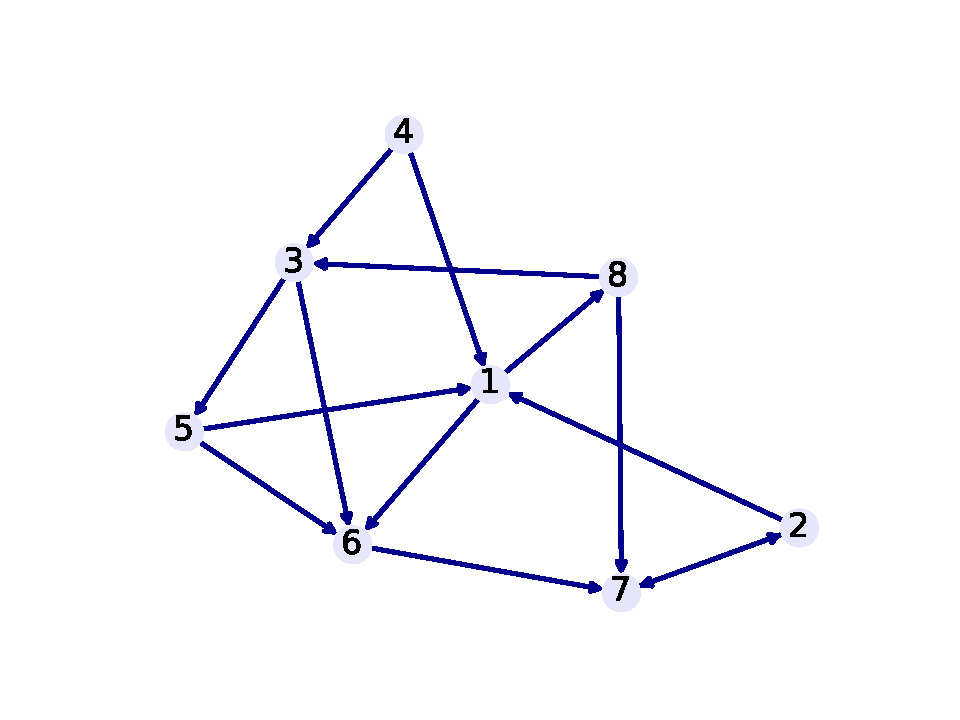
\includegraphics[width=0.9\textwidth]{Plots/graph_example}
	\end{subfigure}
	\begin{subfigure}{0.5\textwidth}
		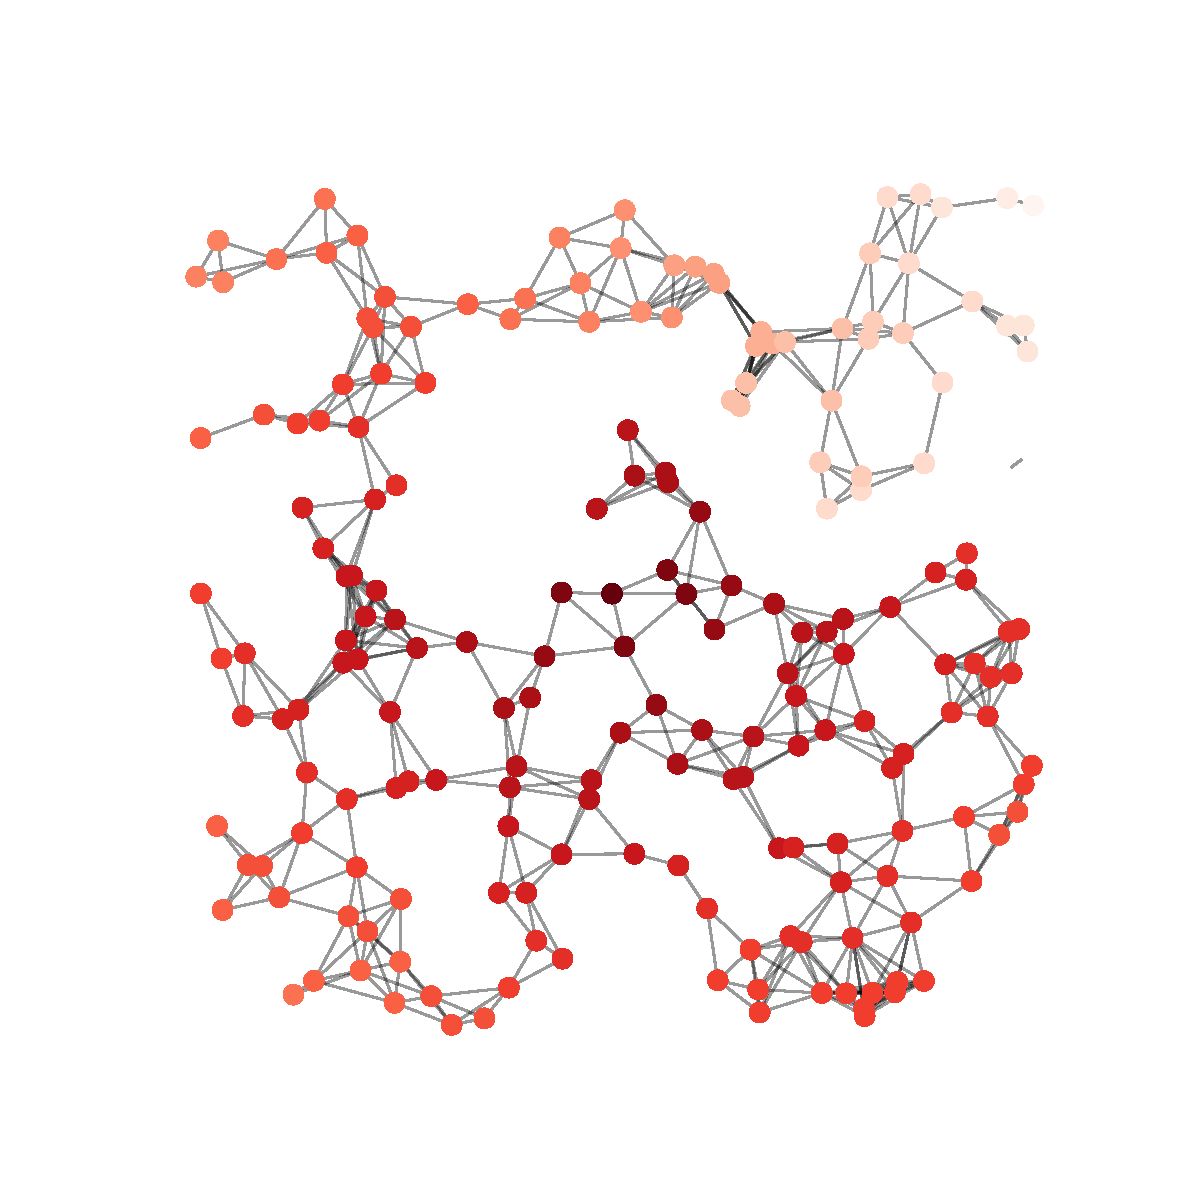
\includegraphics[width=0.8\textwidth]{Plots/graph_example2}
	\end{subfigure}
	\caption{The graph on the left has a total of $ N = 8 $ nodes and degree average of $ k = 1.75$, thus $ 14 $ edges in total. There are two links starting from node $ 1 $ and three pointing towards it, so its degrees are $ k^{(out)}_1 = 2 $ and $ k^{(in)}_1 = 3 $. The graph on the right side is a random geometric graph, which nodes got randomly placed in the plane and if the distance of two happens to be below a certain threshold, an edge was placed between them. Those are only two illustrative examples of graphs and there are uncountable many more.}
	\label{fig:graph_example}
\end{figure}

\paragraph*{Adjacency Matrix}
An introduction to graph theory would not be complete without mentioning the adjacency matrix and its relation to the node degrees. Its elements are defined as
\begin{equation}\label{eq:adjacency_matrix}
A_{ij} =\begin{cases}
1 & \text{if $e_{ij} \in E$}\\
0 & \text{otherwise}.
\end{cases}
\end{equation}
For an undirected graph, we can calculate the in- and out-degree for the $i$-th node as
\begin{equation}
k^{(in)}_i = \sum\limits_{j = 1}^{N} A_{ij} \text{ and } k^{(out)}_i = \sum\limits_{j = 1}^{N} A_{ji}.
\end{equation}
And the number of elements in the set of all edges $ E $ simply is
\begin{equation}
|E| = \sum\limits_{i = 1}^{N} \sum\limits_{j = 1}^{N} A_{ij}.
\end{equation}
For a directed graph, this would count every edge twice. Thus one would have to take half of it to get the right cardinality of the set.


\paragraph*{}
There are numerous ways to select the edges between a given set of vertices to create a network. We could use real-life data to model it or instead randomly select two vertices at a time and connect them until one creates a network with a particular degree distribution. Those distributions are a crucial feature for differentiating between certain types of networks. Typical classes are scale-free, exponential and random graphs. The latest ones often also get called Erd\H{o}s–Rényi models, in honor of the two mathematicians who first introduced and studied them intensively \cite{erdHos1960evolution}.

\paragraph*{}
The random graphs, which are the most important ones for this work, get created by choosing the edges between all nodes with the same probability.
\section{Binary Logic}
\paragraph*{}
In ancient Greek philosophers like Socrates were already asking the ontological question what the essence of reality is and how human beings with all their flaws could possibly know if anything meaningful can understand to be a certain way and not only a product of mankind's imagination. Over two millennia have passed since and such questions are still marveling. Not arguing whether satisfying answers to those mysteries have been found so far or not, it is to acknowledge that many useful theories have been developed in the search for them. Among them are binary logic and information theory, two fields on which modern days technologies strongly depend.

\paragraph*{Boolean Variables}
Binary or often also called Boolean logic is the field that only distinguishes between two truth values: "false" and "true". To make things easier they are often represented as $ 0 $ for false and $ 1 $ is true. Without the necessity of having a semantic meaning, one can obtain reasonable rules for dealing with propositions as such. For example, assume to have a preposition or rather a Boolean variable $ A \in \{0,1\}$. A tautology $ \top $ is a statement that happens to be true no matter which actual values the underlying variables take. One of those is the statement "$ A $ or not $ A $", which is self-evidently true since there are no other choices within the binary framework of logic. The opposite of is a contradiction $ \bot $ like "$ A $ or not $ A $".

\paragraph*{Interpretation and Logical Operators}
A sentence is the combination of propositions with some logical operators. In order to give some examples, it is sufficient to first introduce the interpretation of a proposition or a sentence $ A $:
\begin{equation}
|A| := \begin{cases}
0 & \text{if $A$ is false}\\
1 & \text{if $A$ is true.}
\end{cases}
\end{equation}
This might seem to be a trivial thing to do, but with this it is possible to define logical operators in an arithmetical way. The negation is a compound sentence with one logical operator $ \neg $ which acts on a single proposition $ A $ and its truth value can be calculated to be:
\begin{equation}
|\neg A| := 1 - |A|.
\end{equation}
\paragraph*{}
With a set of only a few logical operators, it is possible to construct all other logical operators. In fact, actually a single one is enough to create every single one of them. But to understand this, it is easier to start from a different point and first define two other logical operators, which now act on two propositions $ A $ and $ B $:
\begin{align}
\text{logical "and" or conjuction:}\quad\quad |A \land B| &:= |A|\cdot|B|, \\
\text{logical "or" or disjunction:}\quad\quad |A \lor B| &:= 1-(1-|A|)\cdot (1-|B|).
\end{align}

\paragraph*{}
To construct an arbitrary logical operator of $ N \in \mathbb{N} $ propositions $ \mathcal{O}(A_1,\dots,A_N) $ one would start by considering all the combinations of truth values, which should make the operator true and connect them with the operators introduced so far. How this should be done, can be most easily demonstrated by an example. The "exclusive or" is the operator $ \oplus $, which is true if either one of its two propositions is true, but false if all of them are false or all of them are true:
\begin{equation}\label{eq:XOR}
|A_1\oplus A_2| := 
\begin{cases}
0 \quad\text{if } |A_1\land A_2| = 1 &(P1),\\
1 \quad\text{if } |\neg A_1\land A_2| = 1 &(P2),\\
1 \quad\text{if } |A_1\land \neg A_2| = 1 &(P3),\\
0 \quad\text{if } |\neg A_1\land \neg A_2| = 1 &(P4).
\end{cases}
\end{equation}

\paragraph*{}
Obviously $ |A_1\oplus A_2| $ is true, if either $ P2 $ or $ P3 $ are the case, which directly leads to another possible way of defining the operator in terms of:
\begin{equation}
|A_1\oplus A_2| = |P2\lor P3| = |(\neg A_1\land A_2)\lor (A_1 \land \neg A_2)|.
\end{equation}

\paragraph*{Adequate Sets}
With this receipt of building disjunctions of conjunctions that are true, one can easily now construct also every other logical operator. This is exactly the definition of functional (or also logical) completeness for a set of logical operators, which are in this case $ \{\neg,\land,\lor\} $. Sets that have this property are then called adequate sets. It is possible to have even smaller logical complete sets of operators. If you consider, that it is $ |A_1\lor A_2|\Leftrightarrow|\neg(\neg A_1\land\neg A_2)| $, which is basically De Morgan's law, then it follows directly, that $ \{\neg,\land\} $ is also an adequate set.

\paragraph*{}
It is even possible to have logically complete sets with only one operator. Peirce's arrow $ \downarrow $ for example is only true, if both of its propositions are false. With this definition it is not too hard to check for the two propositions $ A_1 $ and $ A_2 $, that:
\begin{align}
|\neg A_1| \quad &\Leftrightarrow\quad |A_1 \downarrow A_1|,\\
|A_1\land A_2| \quad &\Leftrightarrow\quad |(A_1\downarrow A_1)\downarrow(A_2\downarrow A_2)|.
\end{align}

\paragraph*{}
This means, that the set $ \{\downarrow \} $ is also complete. Another such an example with only one operator, would be the set with only the so called Sheffer's stroke $ \{\uparrow\} $. They correspond to the NOR and NAND gates of digital electronics and their functional completeness is one of the reasons why they are useful for designing computer processors.


\paragraph*{}
With all those previous definitions, one could basically build every logical sentence and they would syntactically make sense, but it would be rather tedious and inefficient. Thus it is beneficial to introduce some other concepts for working in the field of logic and one very important tool for dealing with logical compositions are truth tables. The interpretations of all possible combinations of the involved logical propositions or, as we will from now on prefer them to call, Boolean variables get written down and besides them, which truth value each finally takes. Table \ref{tab:two_dim_fun} is an example for all the combinations that are possible with up to two binary variables.

\begin{table}
	\centering
	\resizebox{\columnwidth}{!}{%
	\begin{tabular}{|c|c"c|c||c|c|c|c||c|c|c|c|c|c|c|c||c|c|}
		\hline 
		\multicolumn{2}{|c"}{\small $ \sigma $} & \multicolumn{2}{c||}{\small$ \mathcal{A}\ \  $} & \multicolumn{4}{c||}{\small $ \mathcal{B}_1 $} & \multicolumn{8}{c||}{\small $ \mathcal{B}_2 $} & \multicolumn{2}{c|}{\small $ \mathcal{\ C} $}  \\ 
		\hline
		\scriptsize
		$p$ & \scriptsize$q$ & \scriptsize$ \top $ & \scriptsize$ \bot $ & \scriptsize$ p $ & \scriptsize$ \neg p $ & \scriptsize$ q $ & \scriptsize$ \neg q $ & \scriptsize$ p \downarrow q $ & \scriptsize$ p \nleftarrow q$ & \scriptsize$ p \nrightarrow q $ & \scriptsize$ p \land q $ & \scriptsize$ p \lor q $ & \scriptsize$ p \leftarrow q $ & \scriptsize$ p \rightarrow q $ & \scriptsize$ p \uparrow q $ & \scriptsize$ p \leftrightarrow q $ & \scriptsize$ p \oplus q $ \\ 
		\thickhline
		\small 0 & \small 0 & \small 1 & \small 0 & \small 0 & \small 1 & \small 0 & \small 1 & \small 1 & \small 0 & \small 0 & \small 0 & \small 0 & \small 1 & \small 1 & \small 1 & \small 1 & \small 0 \\ 
		\hline 
		\small 0 & \small 1 & \small 1 & \small 0 & \small 0 & \small 1 & \small 1 & \small 0 & \small 0 & \small 1 & \small 0 & \small 0 & \small 1 & \small 0 & \small 1 & \small 1 & \small 0 & \small 1 \\ 
		\hline 
		\small 1 & \small 0 & \small 1 & \small 0 & \small 1 & \small 0 & \small 0 & \small 1 & \small 0 & \small 0 & \small 1 & \small 0 & \small 1 & \small 1 & \small 0 & \small 1 & \small 0 & \small 1 \\ 
		\hline 
		\small 1 & \small 1 & \small 1 & \small 0 & \small 1 & \small 0 & \small 1 & \small 0 & \small 0 & \small 0 & \small 0 & \small 1 & \small 1 & \small 1 & \small 1 & \small 0 & \small 1 & \small 0 \\ 
		\hline 
	\end{tabular} } \par
\vspace{0.3cm}
	\caption{The left two rows show the variables $ p $, $ q $ and below them the truth values they can take. Class $ \mathcal{A} $ are the tautology $ \top $ and contradiction $ \bot $, which actually do not depend on a variable. The identities ($ p $, $ q $) and negations ($ \lnot p $, $ \lnot q $) can be fully decided in terms of only one of the variables. The last two Classes depend actually on both. }
	\label{tab:two_dim_fun}
	
\end{table}

\paragraph*{Boolean Functions}\label{sec:binary_logic}
This style of defining the logical operators is very similar to the one used in the definition of equation (\ref{eq:XOR}). Those operators can also be interpreted as Boolean functions, as will be done in the following section. Such a function is defined as a map, that takes a set $ N $ Boolean variables $ \{\sigma_1,\dots , \sigma_N\} $ and returns a truth value as the result. Formally it is $ f:\{0,1\}^N \longrightarrow \{0,1\} $ with $ ( \sigma_1 , \dots , \sigma_N ) \mapsto f( \sigma_1 , \dots , \sigma_N )$. The values of the $ N $ variables can be combined in exactly $ 2^N $ different ways and every one of them maps either to $ 0 $ or $ 1 $, therefore there exists a total of $ 2^{2^N} $ possible Boolean functions for them. Two variables give as such rise of $2^{2^2}=2^4= 16 $ functions, which can be divided into different classes:
\begin{itemize}
	\item[$ \mathcal{A} $\ ] constant functions -- do not depend on its input values
	\item[$ \mathcal{B}_1 $] fully canalizing functions -- have one relevant input value
	\item[$ \mathcal{B}_2 $]  normal canalizing functions -- some outputs depend on both input values, the others just on one
	\item[$ \mathcal{C} $\ ] non-canalizing functions -- both input values are relevant
\end{itemize}

\paragraph*{}
The classes $ \mathcal{A} $ and $ \mathcal{B}_1 $ are actually the functions that were known with zero and one argument, only  $ \mathcal{B}_2 $ and  $ \mathcal{C} $ do actually depend on both their inputs. With three variables there exist already 256 different Boolean functions, so it would not make any sense to describe them in more detail or try to divide them into different classes. Furthermore, as already has been argued before it is possible to construct every function by combining the ones that are already known with only two arguments.

\section{Boolean Networks}
\paragraph*{}
How does all this previously described come now together in the theory of Boolean Networks (BN)? In principle, a BN is a time-discrete system on a graph. The nodes become the Boolean variables applied to a Boolean function, in which the in-coming edges determine its arguments. The time evolution comes from using those functions on the variables repeatedly. Of course, that is not all there is to it and the details are as always necessary, thus this section will try to give an overview of the whole topic and be more specific about the points that matter most to understand the main results of this thesis.

\paragraph*{}
The RBN consists out of $N$ Boolean variables $ \sigma_i \in \{0,1\} $, with $ i \in \{1,\dots, N\} $. The whole state of the network at time $ t $ is simply the set of all variables $ \Sigma_t = \{ \sigma_1(t),\dots,\sigma_N(t)\}$. The next time step for every variable gets evaluated by using binary coupling functions and determining their value by the links that connect to it - so for the $ i $-th variable, assuming it has $k$ links connecting to it, this would be:
\begin{align}
\sigma_i(t+1)=&f_i(\sigma_{j_1}(t),\dots,\sigma_{j_k}(t))\in \{0,1\},\\
\ with\ j_1, \dots, j_k \in \{1,&\dots,N\}\ and\ \forall l,m \in\{1,\dots,N\}:j_l\neq j_m.
\end{align}

\paragraph*{}
As we can see the value of our $ i $-th variable at time $ t+1 $ depends on the values of all nodes at time $ t $, that point towards it. For our work we used a synchronous update rule, where we apply the next step change to all the variables simultaneously. 

\paragraph*{}
Connecting this with the previously mentioned networks is fairly simple. One determines the dependencies of the variables by the network connections. For example, if in a given configuration there exist the edges $ e_{12} $ and $ e_{14} $, then the function for $ v_1 $ would be: $ \sigma_1(t+1) = f_1(\sigma_2(t),\sigma_4(t)) $. In order to gain further insight, we will consider the following graph with a corresponding set of Boolean functions:

\begin{figure}[h!]
\begin{subfigure}{0.3\textwidth}
\begin{flushright}
\begin{tikzpicture}[x=3cm, y=3cm]
\vertex (ul) at (0,1) {$\sigma_1$};
\vertex (ur) at (1,1) {$\sigma_2$};
\vertex (ll) at (0,0) {$\sigma_3$};
\vertex (lr) at (1,0) {$\sigma_4$};
\draw [->,thick] 
(ur) edge (ul)
(ul) edge (ll)
(ll) edge (lr)
(lr) edge (ur)
(ur) edge (ll)
(lr) edge[bend right=10] (ul)
(ul) edge[bend right=10] (lr);
\draw [->,thick] (ur) to [out=20,in=70,looseness=8] (ur);
\end{tikzpicture}	
\end{flushright}

\end{subfigure}
\begin{subfigure}{0.7\textwidth}
\begin{align}
f_1(\sigma_2,\sigma_4) & = |\sigma_2 \lor \sigma_4| = 1-(1-|\sigma_2|)(1-|\sigma_4|),\\
f_2(\sigma_2,\sigma_4) & = |\sigma_2 \rightarrow \sigma_4| = 1-|\sigma_2|(1-|\sigma_4|),\\
f_3(\sigma_1,\sigma_2) & = |\lnot \sigma_2| = 1 - |\sigma_2|,\\
f_4(\sigma_1,\sigma_3) & = |\sigma_1 \oplus \sigma_3| = |\sigma_1|(1-|\sigma_3|)+(1-|\sigma_1|)|\sigma_3|.
\end{align}
\end{subfigure}
\end{figure}


\paragraph*{}
The adjacency matrix of this graph is:
\begin{equation}
A =
\begin{bmatrix}
0 & 1 & 0 & 1 \\
0 & 1 & 0 & 1 \\
1 & 1 & 0 & 0 \\
1 & 0 & 1 & 0
\end{bmatrix}
\end{equation}

\paragraph*{}
One of the first things we notice is that loops in the graph are possible. Thus the function $f_2$ depends on the value of $\sigma_2$. Another thing is that even though $f_3$ is said to be a function of the variables $\sigma_1$ and $\sigma_2$, it depends only on $\sigma_2$.  So we could remove the edge $e_{31}$ and the dynamics of the whole system would remain the same. Let us consider this example a little bit further and see what else we can learn from it. We start by initializing the variables with values and choose them to be all zero. We can write this as a string in the form of $|\sigma_4||\sigma_3||\sigma_2||\sigma_1|$, which would be in our case $0000$. To calculate the next time-step, one goes through all the functions:
\begin{align}
f_1(0,0) & = 1-(1-0)(1-0) = 0,\\
f_2(0,0) & = 1-0\cdot(1-0) = 1,\\
f_3(0,0) & = 1 - 0 = 1,\\
f_4(0,0) & = 0\cdot(1-0)+(1-0)\cdot 0 = 0.
\end{align}

\paragraph*{}
Notice that even though $f_2$ would have changed the value of $\sigma_2$, we used its old one for $f_3$. This way of updating the state is called synchronous because all the functions are calculated simultaneously. We will always do it like this. Another possibility would be to pick one vertex randomly at a time and only update its variable. It would be the asynchronous method, but this is not of our interest from here on, since the system would no longer be deterministic.
After the update, the new string reads $0110$ or as its integer representation $6$, if we interpret it as a binary number.\footnote{Converting a binary string $n_N\cdots n_1$, with $n_i\in\{0,1\}$ for all $i\in\{1,\dots,N\}$ into decimal can straightforward be calculated as the sum $\sum\limits_{i = 0}^N n_i 2^i$.} Continuing with the update process over and over again creates the following chain:
\begin{equation}\label{eq:cycle3}
0 \rightarrow 6 \rightarrow 9 \rightarrow 15 \rightarrow 3 \rightarrow 9 \rightarrow 15 \rightarrow 3 \rightarrow 9 \rightarrow \dots\ .
\end{equation}

\paragraph*{}
After some steps, the states start to repeat themselves and will not leave the arrived cycle anymore. Thus one would now go ahead and initialize the system ones again, preferably with a state that we did not already have in the path above. The next unvisited integer value would be $1$ and if we start with it, we get:
\begin{equation}\label{eq:cycle1}
1 \rightarrow 14 \rightarrow 11 \rightarrow 11 \rightarrow 11 \dots\ .
\end{equation}

\paragraph*{}
Applying the update rule to the state $11$ leads again to itself. Thus when we compare it with the definition in equation (\ref{eq:fixpoint}), we can conclude that we found a fixpoint. All this means we have at least two separate paths that will never cross each other. If one goes through all other states, they would either lead to the cycle in equation (\ref{eq:cycle3}) or the fixpoint in equation (\ref{eq:cycle1}). What does this tell us now about the dynamics of a BN?

\paragraph*{}
Remember that the collection of all possible states the network can be in is the phase space. For a BN of size $ N $, there are exactly $ \Omega = 2^N $ different states. In the example, this would have been $16$. When a system with only a finite-sized phase space evolves over time, it will inevitably come to a state it already has been in and thereon repeating the path up to itself again on a cycle. The number of states a cycle contains is called its length and will be denoted by $ L $. 

\paragraph*{Attractors}
We now call an attractor a cycle that can be reached from states that are not part of itself, analogous to a contracting phase space of continuous dynamical systems. Since finding a cycle that is not also an attractor is pretty rare, we will not distinguish between the two. Attractors of length $ L=1 $ are also often referred to as fixpoints. All states that lead to an attractor plus its cycle elements are called the basin of attraction. We denote its number by $ \mathcal{N}_B $. In the literature, those are also called modules, as in \cite{aldana2003boolean}. All in all, this means that we have found in the example network two different attractors with lengths $3$ and $1$.

\begin{figure}[t]
	\centering
	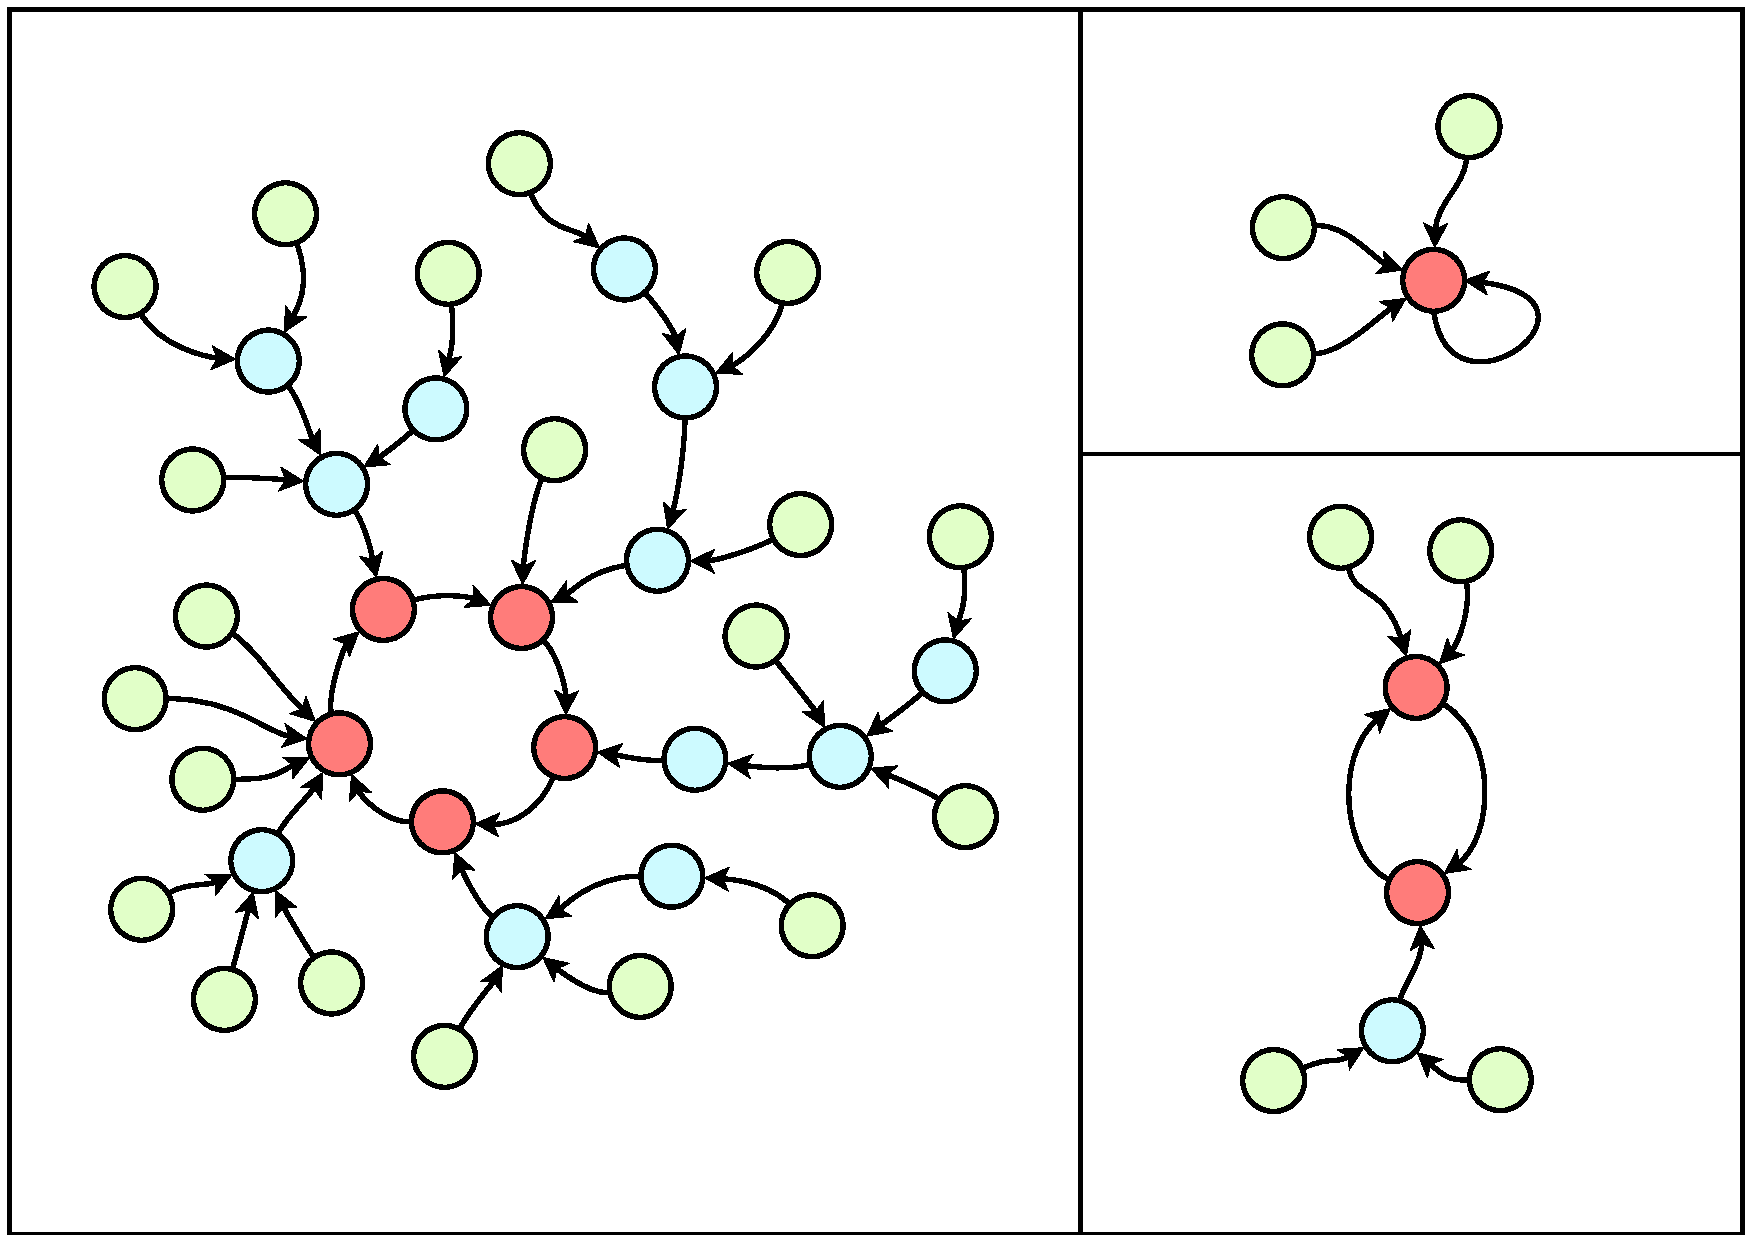
\includegraphics[width=0.7\textwidth]{Plots/phase_space}
	\par
	\vspace{0.3cm}
	\caption{This figure is the schematic representation of a finite-sized phase space of any time-discrete and deterministic system. Every circle is a possible state $ \Sigma $ in phase space. The arrows go to the next state to which the current step leads after a single time step. Here the system has three attractors, sometimes also called modules in the literature. The red circles are states of their so-called cycles, which will repeat themselves over and over again. On the left side is an attractor with five red states. Thus it is said to have a length $ L $ of five. In light green, we have the garden-of-Eden states and all states that lead to the same cycle, plus its states themselves are the basin of attraction.}
	\label{fig:phase_space}
\end{figure}

\paragraph*{Garden-of-Eden States}\label{sec:garden-of-Eden}
A state without predecessor is called garden-of-Eden state. The G-density $\Gamma$ is defined as the fraction those $\mathcal{N}_G$ states are compared to the whole basin of an attractor. A precise definition could not be found throughout the literature, so that we will define it using the following equation:
\begin{equation}\label{eq:g-density}
\Gamma = \left\langle\tfrac{\mathcal{N}_{G}}{\mathcal{N}_{B}}\right\rangle_{\text{Attractors}}.
\end{equation}
So we take the average over all attractors in the system, which is a nice way of doing it generalizes to the case when we have finally introduced random Boolean networks. For a graphical representation of all the previously introduced concepts, see Figure \ref{fig:phase_space}.

\section{Random Boolean Network Ensembles}

\paragraph*{}
This thesis is mainly about the random Boolean network (RBN) model introduced by S. Kauffman in 1969 \cite{kauffman1969homeostasis} and in this section, we will finally introduce the final ideas necessary to comprehend our work. The arguments and derivations here and in the following chapter will mainly follow three sources. The first one to mention is the review from M. Aldana et al. \cite{aldana2003boolean} in which they highlighted the aspects of cycle behavior and information flow in such systems. Secondly, we used the review by B. Drossel \cite{drossel2008random}, from which we gained insights on RBNs up to the level of individual node behavior. And not at least to mention as source the book of C. Gros, in which he gave a broad overview of the topic and comprehensively derived specific properties. Whenever we use something of them or other authors almost one to one, this will be stated explicitly. But for all other cases and to provide a good reading flow, we will refer to them as our primary sources.

\paragraph*{}
One of the main differences to what we have described in the previous section is that we will move away from looking at individual networks and describe fairly large ensembles. Also, until now, there was no randomness involved in all our definitions. So, where does this come into play with RBNs? Exactly twofold: graph structure and choice of Boolean functions.

\paragraph*{Out-degree Distribution}
We are mainly interested in the $ N $-$ K $-Network model, how S. Kauffman defined it in 1969 \cite{kauffman1969metabolic}. In his honor, those networks often are referred to as Kauffman-Networks.  Those are Boolean networks with $ N $ vertices, where each of those has an in-degree of $ k^{(in)} = K $, with a constant $ K \in \{1,\dots,N\} $. Thus, every variable depends on the values of $ K $ randomly chosen nodes. We can calculate the probability distribution of the out-degree $ p_{k}^{(out)} $ as a Bernoulli process. We pick for every node two other ones, so the likelihood of choosing a certain vertex becomes $ p = K/N $. This random choice gets repeated for every node. Thus the probability of having an out-degree of $ k $ becomes:
\begin{equation}\label{eq:Poisson}
p_{k}^{(out)} = {N\choose k}p^k (1-p)^{N-k}\ \ \stackrel{1\ll N}{\longrightarrow}\ \ \frac{K^k e^{-z}}{k!}.
\end{equation}

\paragraph*{}
This is just the Bernoulli process, for which we defined the probability in equation (\ref{eq:Bernoulli}). The right side is an approximation for very large $ N $. This is the so-called Poisson distribution and it can be derived like C. Gros \cite{gros2010complex} showed it in his book in the chapter on graph theory. Suppose we have a very large $ N $, from which immediately follows a small $p=\tfrac{K}{N}$. Then the following approximations can be made and thereby also the one in equation (\ref{eq:Poisson}) holds for all finite node degrees $ k $:
\begin{equation}
{N\choose K} = \frac{N!}{k!(N-k)!} \simeq \frac{N^k}{k!},\ \ \ \ \left(1-\frac{K}{N} \right)^N \simeq e^{-K},\ \ \ \ \left(1-\frac{K}{N} \right)^{-k} \simeq 1.
\end{equation}

\paragraph*{}
Of course, one could also go the other way around and construct a given out-degree distribution network. Like R. Serra et al. did, there works \cite{serra2004dynamics} and \cite{serra2008simulation} for a scale-free topology. The distribution for this would be of the form
\begin{equation}\label{eq:scale_free_degree_distribution}
p_k^{(out)} = \frac{1}{\zeta(\gamma)}k^{-\gamma}\text{, with } \zeta(\gamma)= \sum\limits_{k=1}^{k_{max}}k^{-\gamma}.
\end{equation}

\paragraph*{}
Since we allow self-coupling, it would be $k_{max}=N$. Thus, for $N\longrightarrow \infty$ the $\zeta(\gamma)$ is just the Riemann-zeta function. In the exponent, we have the so-called scaling parameter $\gamma$ that is as far as we are interested, just a real value greater than one. Now you would construct a graph that obeys this distribution. We will not discuss how this would have to be done, since this is more of a side note. There are reasons one could choose such a topology over what we have described before, which could come from observations in the natural world. But since we are more interested in the model, we will stick to the way that constructs networks most randomly. In fact, if you consider large enough ensembles, they will contain all kinds of different topologies. As such, the scale-free networks are also part of our studies. We simply do not favor them over others. Another thing would be to vary the in-degree of the network, which we will have to do when the average degree $K$ is not an integer.

\paragraph*{Coupling Functions}
There are a couple of ways to decide on the coupling functions, once the network structure has been determined. We will here just present them in a similar fashion to the one of B. Drossel \cite{drossel2008random} in her review:
\begin{itemize}
	\item[-] Magnetization bias: We introduce the probability $p$ with which we choose a $ 1 $ as the output of the function for a given set of input values. With two input variables, for example, the implication $\sigma_i \rightarrow \sigma_j$ would then appear with the probability $ p^3(1-p) $, since it becomes only $0$ when $\sigma_i = 1$ and $\sigma_j = 0$. Generally speaking, if a function has $M$ outcomes with probability $ p^n (1-p) ^{M-n} $, we would pick a function with $ n $ ones. The most equally distributed choice and the one S. Kauffman used to introduce the model would be $ p=0.5 $.
	\item[-] Weighted classes: When we divide the possible binary functions into different classes as we did for two variables in section \ref{sec:binary_logic}, we can introduce weights for each class, with which we will take one of this class. For $n$ different classes, we pick the weights $ w_1 \dots w_n $ for every one of them. As they must be proper weights, they fulfill $ \sum w_i =1 $ and all of them are $w_i \in [0,1]$. The weighted method could be useful when someone finds that natural networks tend to prefer a certain class of functions. As seems to be the case with gene regulatory networks, which tend to be more often canalizing functions, see \cite{harris2002model} or \cite{kauffman2003random}. 
\item[-] Threshold functions: We could be interested in modeling some properties of firing neurons and therefore decide to use functions that only activate if enough input states are active. We then define the function for the $i$-th vertex with $ n $ in-going edges as:
\begin{equation}
f(\sigma_{i_1},\dots , \sigma_{i_n}) = \begin{cases}
1 &\text{if } \sum\limits_{j=1}^{n}\sigma_{i_j}>h,\\
0 &\text{else},
\end{cases}
\end{equation}
	where $ h $ would be a threshold greater than zero.
	\item[-] Cellular automaton with random couplings: We assign to every vertex the same coupling function.
\end{itemize}

\paragraph*{}
As before with the topology decision, all other cases would be interesting to study on their own, but the focus of our attention will be the magnetization bias method.

\paragraph*{Number of possible RBNs}
I. Harvey and T. Bossomaier \cite{harvey1997time} estimated the number of all possible RBNs with $N$ vertices and the in-degree $ K $ in the following way. You have to choose $ K $ other nodes for one of them, leading to $ N!/\left[K!(N-K)!\right]  $ possible ways of doing this. Then there are $ 2^{2^K} $ possible coupling functions, as we explained in section \ref{sec:binary_logic}. Since this has to be done for all $ N $ vertices, it is clear that the number of all possibilities becomes 
\begin{equation}
\left[2^{2^K}{N\choose K}\right]^N .
\end{equation}

\paragraph*{}
This entails even for fairly small networks a huge amount of possibilities. For example, say we have $N = 4$ and $K = 2$, leading to a number of $8.49\cdot 10^7$ rounded. Of course, one could argue that this estimation is a little bit far fetched. If you have a given network and change the outcome for every boolean function from $0$ to $1$ and the other way around, you may have a different network. But from a dynamical point of view, their behavior is identical. Another argument for a smaller estimate would be that there is no difference between the nodes. Thus there will be topologically equivalent networks. Both of these points would reduce the total count of different networks by some amount. But for all practical purposes, this is irrelevant since there is no practical way of determining whether a network is in principle the same in a somewhat large ensemble of them yet.

\paragraph{Ensambles, Mean Values and Variance}
An ensemble is a collection of several randomly initialized network realizations. More precisely, we will work most of the time with ensemble averages. If we are interested in some value, like the number of attractors $ \mathcal{N}_A $ in the RBNs of a certain kind, we store their values in a set $\mathcal{S}$. With $|\mathcal{S}|$ realizations, we will get the values $\mathcal{N}_A^{(1)},\dots,\mathcal{N}_A^{(|\mathcal{S}|)}$ and can take their ensemble average as:
\begin{equation}
\langle \mathcal{N}_A \rangle := \langle \mathcal{N}_A \rangle_\mathcal{S} := \frac{1}{|\mathcal{S}|} \sum\limits_{i=1}^{|\mathcal{S}|} \mathcal{N}_A^{(i)}.
\end{equation}
Whenever it is clear on which set the average gets taken, we can omit to write it down besides the right angle. The variance is a measure on how much the individual found values differ from this average, thus it is defined as:
\begin{equation}
\sigma^2 = \langle (\mathcal{N}_A-\langle \mathcal{N}_A \rangle)^2 \rangle.
\end{equation}
Taking the squareroot of this gives us the so-called standard deviation $ \sigma $.

\paragraph*{Hamming Distance}
The Hamming distance is a tool for measuring differences between two strings of information of equal length. For two states $ \Sigma $ and $ \tilde{\Sigma} $ it is defined as:
\begin{equation}\label{eq:hamming_distance}
D(t) = \sum\limits_{i = 1}^N \left( \sigma_i(t) - \tilde{\sigma}_i(t) \right)^2.
\end{equation}
For RBNs, we need it in order to measure how much information the system preserves over time. If we consider this to be a distance, we can ask ourselves if it will grow over time for two close, but not identical, initial states.

\paragraph*{}
We could define many more things concerning the dynamics of RBNs right now, but they seem to be more fitting in the context of our research. Thus, we will introduce them in the next chapter, when they actually appear to be needed. By now, we should have gained a clear picture of the model we are using and all the necessary mathematical background it was built on.

\paragraph*{Ergodic Sets}\label{sec:ergodic_set}
Ergodic sets were already proposed in 1969 by S. Kauffman himself, who thought them to be a good candidate for representing different cell types \cite{kauffman1969metabolic}. They are defined as the transition network that gets created by flipping single nodes in an attractor and connecting two of them, if such a change leads from the first ones cycle to the second. By now we know, that they themselves are not as useful as they were suspected to be for representing cell types, since most networks appear to have only a single ergodic set, like A. Ribeiro and S. Kauffman himself elaborated in \cite{ribeiro2007noisy}. 

\paragraph*{}
Ergodic sets are closely related to the topic of attractor robustness at which we also look in our work though we will prefer the name attractor stability for it. The robustness has often been of interest in studying random Boolean networks and can, for example, be found in works from B. Luque et al. \cite{luque1998stable}, or K. Willadsen et al. \cite{willadsen2008understanding}. We will later introduce the certain notion of attractor stability in which we are interested in.

\newpage\thispagestyle{empty}